\documentclass[11pt]{article}   % tipo de documento e tamanho das letras

% os seguintes pacotes estendem a funcionalidade básica:
\usepackage[a4paper, total={16cm, 24cm}]{geometry} % tamanho da pagina e do texto
\usepackage[portuguese]{babel}  % traduz para portugues
\usepackage[utf8]{inputenc}
\usepackage{graphicx}           % graficos
\usepackage{amsmath}            % matematica
\usepackage{tikz}               % diagramas
    \usetikzlibrary{shadows}
\usepackage{booktabs}           % tabelas com  melhor aspecto
\usepackage[colorlinks=true]{hyperref}           % links para partes do documento ou para a web
\usepackage{listings}           % incluir codigo
    \renewcommand\lstlistingname{Listagem}  % Listing em portugues
    \lstset{numbers=left, numberstyle=\tiny, numbersep=5pt, basicstyle=\footnotesize\ttfamily, frame=tb,rulesepcolor=\color{gray}, breaklines=true}
\usepackage{blindtext}

% -------------------------------------------------------------------------------------------
\title
{
    
\includegraphics[width=0.3\textwidth]{images/logo_universidade.png}
    \\[0.1cm]
    \textbf{Simulador de Escalonamento de Processos} \\
    Sistemas Operativos I
}

\author
{
    \textbf{Professor:} Luís Rato \\
    \textbf{Realizado por:} Miguel de Carvalho 43108 
}
\date{3 de Abril de 2020}

% -------------------------------------------------------------------------------------------
%                                Body                                                       %
% -------------------------------------------------------------------------------------------

\begin{document}
\maketitle

% -------------------------------------------------------------------------------------------
\section{Introdução} 

\hspace{0,5cm}Neste trabalho foi solicitado a realização de um programa que simule o \textbf{Escalonamento de Processos} num modelo de 3 estados. Na figura abaixo está representado o diagrama que descreve o modelo de 3 estados:\par
\begin{figure}[h!]
    \begin{center}
        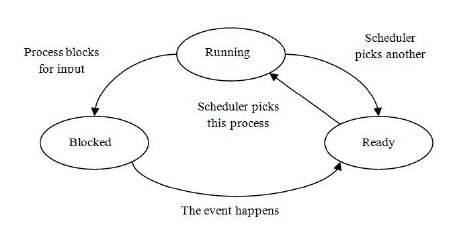
\includegraphics[width=0.8\textwidth]{images/states.png}
        \caption{Diagrama de 3 Estados}
    \end{center}
\end{figure}
O \textbf{Escalonador de Processos} faz parte do \textbf{Sistema Opertivo} e é responsável por decidir em que momento cada processo estará no CPU. 
Existem muitos algoritmos de escalonamento para realizar essa decisão. \par
\newpage
Neste trabalho serão utilizados o algoritmo \textbf{FCFS} e o \textbf{Round Robin (RR)}:
\begin{itemize}
    \item O \textbf{FCFS} é um algoritmo de escalonamento não preemptivo que prioriza os processos pela ordem de chegada. Executa o processo todo do inicio ao fim sem o interromper, até estar concluído. Quando aparece um novo processo e ainda existe um em execução, esse novo irá para a fila de espera.
    \item O \textbf{Round Robin (RR)} é um algoritmo de escalonamento preemptivo que apresenta um funcionamento igual ao do \textbf{FCFS}, mas com tempo limite de execução, o \textbf{Quantum}. Ou seja, quando o processo se encontra em execução este irá ser interrompido quando o tempo de execução for igual ao /textbf{Quantum} e irá para a fila de espera (/textbf{READY}) 
\end{itemize}

% -------------------------------------------------------------------------------------------
\section{Implementação}

\hspace{0,5cm}Primeiramente comecei por pensar como deveria proceder para realizar o trabalho, e na primeira tentativa comecei por desenvolver o \textbf{FCFS}, mas na segunda tentativa cheguei a conclusão de que não seria necessário realizar um programa para a implementação do \textbf{FCFS} e outro para o \textbf{Round Robin}, pois ambos são iguais, execto existir um limite de execução no \textbf{RR}. \par
Poderei então meter um limite muito grande na execução, no \textbf{Quantum}, e estarei perante o FCFS. \par
Comecei por proceder há criação das queues que iriam ser utilizados para o \textbf{READY}, \textbf{RUN} e \textbf{BLOCKED} e das respetivas funções essenciais para a sua manipulação. \par
O próximo desafio foi proceder a leitura do input (ficheiro com os processos e os tempos), para isso foi necessário proceder a criação de uma \textbf{Struct} para os processos.\par
Por conseguinte, comecei por desenvolver a função que iria realizar as trocas dos processos entre os 3 estados. Esta função foi a mais difícil de realizar devido a complexidade dos requísitos para os processos mudarem de estados. Foi necessário também proceder a criação de novas funções para facilitar alguns procedimentos que eram realizados de forma repetitiva.

% -------------------------------------------------------------------------------------------
\section{Execução}

\hspace{0,5cm}Quando o utilizador executar o \textbf{Simulador de Escalonamento} irá ser questionado acerca do nome do ficheiro de input e qual algoritmo pretende utilizar.
\begin{itemize}
    \item Caso o utilizador escolha o \textbf{FCFS}, o \textbf{QUANTUM} irá ter um valor de \textbf{10000}, assim nunca irá obrigar o programa a passar para o estado ready.
    \item Caso o utilizador escolha o \textbf{Round Robin}, será perguntado ao utilizador qual o \textbf{Quantum} desejado.
\end{itemize}
% -------------------------------------------------------------------------------------------
\section{Análise de Resultados} % Conclusão
Em suma, este trabalho fez-me entender melhor como funciona o escalonador e as condições que cada algoritmo usa para proceder há mudança dos processos entre os estados e as diferenças de tempo. 

% -------------------------------------------------------------------------------------------
\section{Problemas}
\hspace{0,5cm}Neste trabalho só existe um problema e consiste no facto de que em algumas execuções o ultimo processo existente no ficheiro não é lido, mas este problema só acontece no \textbf{Linux}. Por outro lado no \textbf{Windows} este problema não ocorre.
% -------------------------------------------------------------------------------------------
\section{Conclusão} % Conclusão
Em suma, este trabalho fez-me entender melhor como funciona o escalonador e as condições que cada algoritmo usa para proceder há mudança dos processos entre os estados e as diferenças de tempo. 
% -------------------------------------------------------------------------------------------
\end{document}